\scanpage{77}
connected, whose $\pi_1$ is isomorphic as an \uline{outer group}) :
\diagram{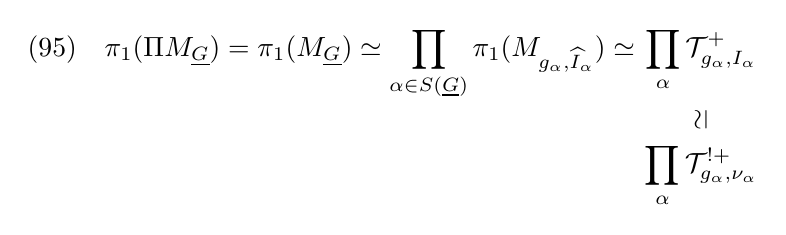
\begin{tikzpicture}[every node/.style={inner sep=0pt}]
\node[anchor=base east] (chain) at (0,0) {$\displaystyle(95)\quad\pi_1(\Pi M_{\underline G})=\pi_1(M_{\underline G})\simeq\prod_{\alpha\in S(\underline G)}\pi_1(M_{g_\alpha,\widehat I_\alpha})\simeq$};
\node[anchor=base west] (upper) at (0.12,0) {$\displaystyle\prod_\alpha\mathcal T^+_{g_\alpha,I_\alpha}$};
\node[rotate=90] at ([yshift=-0.35cm]upper.south) {$\simeq$};
\node[anchor=north] at ([yshift=-0.65cm]upper.south) {$\displaystyle\prod_\alpha\mathcal T^{!+}_{g_\alpha,\nu_\alpha}$};
\end{tikzpicture}}
\margin{where the $\mathcal T^{!+}_{g,\nu}$ are Teichmüller groups}
The actions of $\Gamma^{\unsure{!|\natural|\deleted{!}}}_{\underline G}$ on $\Pi M_{\underline G}$ define a mixed groupoid $(\Pi M_{\underline G},\Gamma_G)$, whose (outer) fundamental group \unsure{fits} \deleted{\unsure{of} \unsure{by}} \inserted{into an} extension structure
\[
(96)\quad1\longrightarrow\pi_1(\Pi M_{\underline G},\Gamma_{\underline G})\longrightarrow\pi_1(\Pi M_{\underline G},\Gamma_{\underline G})\relbar\joinrel\relbar\Gamma_G\longrightarrow1
\]
We shall define a \inserted{sort of} variance of the $\Pi M_{\underline G}$ relative to two sorts of ``morphisms'' for MD-graphs $\underline G$. 

First of all a \uline{``variance of generization''}, which is composed of the \uline{variance for isomorphisms} of MD-graphs (which I accept as ``trivial'', and which it is unnecessary to specify) and a ``variance of passage to the \unsure{quotient} of MD-graphs''.
\margin{76}
